\documentclass[a4paper,11pt]{article}
\usepackage[utf8]{inputenc}
\usepackage{lastpage}
\usepackage{fancyhdr}
\usepackage[english]{babel}
\usepackage[a4paper,margin=1in]{geometry}
\usepackage{multirow}
\usepackage[table,xcdraw]{xcolor}
\usepackage{array}
\usepackage{graphicx}
\usepackage{caption}
\usepackage{ctable}
\usepackage{listings}
\usepackage[T1]{fontenc}
\usepackage{bigfoot} % to allow verbatim in footnote
\usepackage[numbered,framed]{matlab-prettifier}
\usepackage{amsmath}


\newcolumntype{L}[1]{>{\raggedright\let\newline\\\arraybackslash\hspace{0pt}}m{#1}}
\newcolumntype{C}[1]{>{\centering\let\newline\\\arraybackslash\hspace{0pt}}m{#1}}
\newcolumntype{R}[1]{>{\raggedleft\let\newline\\\arraybackslash\hspace{0pt}}m{#1}}

\newcommand\tab[1][4mm]{\hspace*{#1}}


%-------------------------------------------------------------------------------
% HEADER & FOOTER
%-------------------------------------------------------------------------------

\pagestyle{fancy}
\fancyhf{}
\setlength\headheight{15pt}
\fancyhead[L]{ Imaging Lab 6 }
\fancyhead[R]{Student ID: 100633486}
\fancyfoot[R]{Page \thepage\ of \pageref{LastPage}}


%-------------------------------------------------------------------------------
% TITLE PAGE
%-------------------------------------------------------------------------------

\begin{document}

\title{
	\Huge \textbf {The Heat Equation}
    \\ [0.2cm]
	\LARGE Imaging Lab 6 - May, 2017
    \\ [0.5cm]
    \hrule
}

\date{}

\author{
		\Large Kamyar Nazeri \\
		\large Student ID: 100633486 }

\maketitle
\newpage

\section*{Anisotropic Diffusion: Color Images}
According to heat equation, the heat dissipates with the following PDE:
\begin{align*}
u_t = \frac{\partial}{\partial x}(K u_x)
\end{align*}
When $K(x)$ changes throughout the bar, then heat will flow unevenly and we call this anisotropic diffusion and the 2D PDE becomes:
\begin{align*}
u_t = \nabla \cdot (K \nabla u) = \frac{\partial}{\partial x}(K u_x) + \frac{\partial}{\partial y}(K u_y)
\end{align*}
For conductivity function \emph{K} we use Perona-Malik exponential edge-stopping function:
\begin{align*}
K = e^{-(\Vert\nabla u\Vert/a)^2}
\end{align*}
Where 
\begin{align*}
\Vert\nabla u\Vert = \sqrt{u_x^2 + u_y^2}
\end{align*}
\\Temporal discretization of the PDE is:
\begin{align*}
u^{n+1} = u^n + \Delta t\ \big[\frac{\partial}{\partial x}(K u_x^n) + \frac{\partial}{\partial y}(K u_y^n)\big]
\end{align*}
 \\
To apply anisotropic diffusion on a color image, we calculate the equation above on each of the 3 RGB channels and storing it in the corresponding channel of a new image. As the first step inside the for loop, we calculate the forward differences to approximate the first
derivatives $u_x$ and $u_y$: 
\begin{align*}
u_x \approx D_x^{+}u = u(x+1,y)-u(x,y) \\
u_y \approx D_y^{+}u = u(x,y+1)-u(x,y) \\
\end{align*}
And to calculate $\frac{\partial}{\partial x}(K u_x)$ and $\frac{\partial}{\partial y}(K u_y)$ we perform forward then backward differences:
\begin{align*}
\frac{\partial}{\partial x}(K u_x) \approx D_x^{-}(KD_x^{+}u) \\
\frac{\partial}{\partial y}(K u_y) \approx D_y^{-}(KD_y^{+}u) \\
\end{align*}
Finally the PDE becomes:
\begin{align*}
u^{n+1} = u^n + \Delta t\ \bigg[D_x^{-}\Big(e^{-(\Vert\nabla u^n\Vert/a)^2} D_x^{+}u^n\Big) + D_y^{-}\Big(e^{-(\Vert\nabla u^n\Vert/a)^2} D_y^{+}u^n\Big)\bigg]
\end{align*}
\\We use Forward Euler Method with Neumann boundary conditions to solve the above equation.

\newpage
\section*{Coding Anisotropic Diffusion}
\emph{Listing 1} shows the anisotropic diffusion applied on a color image in Matlab:
\begin{lstlisting}[caption={Anisotropic Diffusion for Color Images in Matlab},captionpos=b,style=Matlab-editor]
clear;
img = imread('peppers.png');

%Parameters
a = 25;                 % Edge-stopping
dt = 0.1;               % Time step
T = 20;                 % Stopping time
K = 0;                  % Conductivity
[m,n,c] = size(img);    % Image size

%Initialize: convert to double so we can do arithmetic.
res = double(img);

for t = 0:dt:T
    for c=1:3
        % read image channel (RGB)
        u = res(:,:,c);
        
        % u_x forward difference: u(x+1,y) - u
        u_x = u(:,[2:n,n]) - u;
        
        % u_y forward difference: u(x,y+1) - u
        u_y = u([2:m,m],:) - u;
        
        % norm of the gradient
        norm = sqrt(u_x.^2 + u_y.^2);
        
        % Perona-Malik exponential edge-stopping
        K = exp(-(norm./a).^2);

        % backward difference u_x(K.u_x)
        p_x = K .* u_x;
        p_x = p_x - p_x(:,[1,1:n-1]);       

        % backward difference u_y(K.u_y)
        p_y = K .* u_y;
        p_y = p_y - p_y([1,1:m-1],:);

        % anisotropic forward euler
        res(:,:,c) = u + dt * (p_x + p_y);
    end
end

imshow(uint8(res)); 

\end{lstlisting}

\newpage

\emph{Figure 1} shows a test image and two diffused images for different values of Edge-Stopping parameter. As shown below, anisotropic diffusion turns photos into cartoons and the value of \emph{a} controls how diffusion will stop at the edges of the image:

\begin{figure}[!htb]
  \centering
  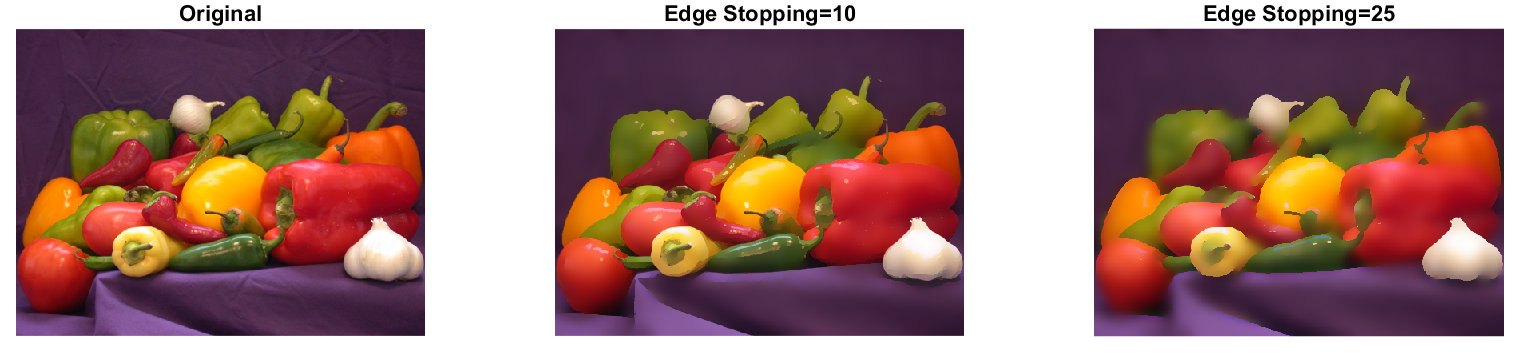
\includegraphics[width=16cm, height=3.7cm]{1.png}
  \caption{\small Anisotropic Diffusion applied on a color image with different Edge-Stopping values.}
\end{figure}

\end{document}
